\documentclass[tikz, border=1mm]{standalone}
\usepackage{amsmath, amssymb}

\begin{document}
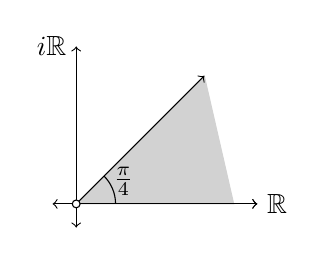
\begin{tikzpicture}[scale=1]
    \draw[fill=gray!35, color=gray!35] (0, 0) -- (2, 0) -- (45:2.3) -- cycle;
    \draw[<->] (-0.3, 0) -- (2.3, 0) node[right]{$\mathbb R$};
    \draw[<->] (0, -0.3) -- (0, 2) node[left]{$i \mathbb R$};

    \draw[->] (0, 0) -- (45:2.3);
    \draw[->] (0, 0) -- (2.3, 0);

    \draw (0:0.5) arc (0:45:0.5) node[xshift=7, yshift=-2]{$\frac{\pi}{4}$};
    \draw (0, 0) node[circle, draw, inner sep=1pt, fill=white]{};
\end{tikzpicture}
\end{document}
